% Bevi -- ranking, scoring and recommendation: mathematical specification.
% Build: tectonic docs/bevi-ranking-math.tex   (or pdflatex twice)
% Source of truth for the implemented parts: packages/ranking/src (RANKING_VERSION 1.3.0).
% Section 10 specifies the extensions discussed on 2026-10-14 (CONVERSATION-2.md, TASKS.md).
% Revised 2026-10-24 (M-22 review): corrections in Sections 2, 3, 5, 6, 8, 9; Sections 10 and 11
% brought up to date with #96, #101, #112, #113, #115, #117, #118 and #121. No version change.
% RANKING_VERSION 1.3.0 (M-28): Section 6.4 (Pearson, taste neighbourhoods), the 1.3.0 row in Section 11.
\documentclass[11pt]{article}
\usepackage[margin=1in]{geometry}
\usepackage{amsmath,amssymb,amsthm,mathtools}
\usepackage{booktabs}
\usepackage{array}
\usepackage{enumitem}
\usepackage{microtype}
\usepackage{xcolor}
\usepackage{algorithm}
\usepackage{algpseudocode}
\usepackage{tikz}
\usetikzlibrary{arrows.meta,positioning,calc,decorations.pathreplacing}
\usepackage[colorlinks=true,linkcolor=blue!55!black,citecolor=blue!55!black,urlcolor=blue!55!black]{hyperref}

\setlist{nosep}
\DeclarePairedDelimiter\floor{\lfloor}{\rfloor}
\DeclarePairedDelimiter\ceil{\lceil}{\rceil}
\DeclarePairedDelimiter\abs{\lvert}{\rvert}
\DeclareMathOperator*{\argmax}{arg\,max}
\DeclareMathOperator{\clamp}{clamp}
\DeclareMathOperator{\simi}{sim}
\DeclareMathOperator{\cosim}{cos}
\DeclareMathOperator{\aff}{aff}
\DeclareMathOperator{\conf}{conf}
\DeclareMathOperator{\supp}{supp}
\DeclareMathOperator{\cat}{cat}
\DeclareMathOperator{\lca}{lca}
\DeclareMathOperator{\depth}{depth}
\DeclareMathOperator{\hot}{hot}
\DeclareMathOperator{\jac}{J}
\newcommand{\code}[1]{\texttt{#1}}
\newcommand{\R}{\mathbb{R}}
\newcommand{\N}{\mathbb{N}}
\newcommand{\ind}[1]{\mathbf{1}\!\left[#1\right]}
\newcommand{\zhat}{\hat{z}}
\newcommand{\shat}{\hat{s}}

\theoremstyle{plain}
\newtheorem{theorem}{Theorem}[section]
\newtheorem{proposition}[theorem]{Proposition}
\newtheorem{lemma}[theorem]{Lemma}
\newtheorem{corollary}[theorem]{Corollary}
\theoremstyle{definition}
\newtheorem{definition}[theorem]{Definition}
\newtheorem{example}[theorem]{Example}
\theoremstyle{remark}
\newtheorem{remark}[theorem]{Remark}
\newtheorem{implnote}[theorem]{Implementation note}

\title{\textbf{The Bevi Ranking and Recommendation System}\\[4pt]
\large Mathematical specification of \code{@bevi/ranking} v1.3.0\\ and the extensions proposed on 2026-10-14}
\author{Bevi (Matt \& Arjun)\thanks{Drafted from \code{packages/ranking/src}, \code{DEVELOPMENT-MATT.md} \S 8 and the second planning session (\code{CONVERSATION-2.md}). Sections 2--9 describe what is implemented and tested; Section 10 specifies the extensions, several of which have since shipped (its introduction says which). Revised on 2026-10-24 after the M-22 review of this paper against the package and the SQL; the review's correction lists are under M-22 in \code{TASKS.md}. Formula changes must bump \code{RANKING\_VERSION} and regenerate the golden vectors in \code{shared/fixtures}.}}
\date{14 October 2026, revised 24 October 2026}

\begin{document}
\maketitle

\begin{abstract}
Bevi asks a user to compare a beverage (``Bev'') against beverages they have already ranked and converts the answers into a personal 0--10 score, a global leaderboard and a prediction of how much a user would like a Bev they have not tried. This document states every formula the system uses, proves the properties the product relies on (termination and correctness of placement, exactness of stored scores, boundedness of predictions), explains the numbers users see (why two ratings of 7.6 and 2.0 display as 5.9), and specifies the extensions agreed in the 14 October 2026 session: category-aware comparisons over a weighted Bev graph (weights from taxonomy, content, text embeddings and flavour profiles, computed into Postgres and mirrored to Neo4j), the Taste Profile, Bev of the day and of the week, likes and an Explore ranking, a Smart Recommend filter for the map, nutrition normalisation and duplicate detection. It closes with the places where the SQL and TypeScript implementations currently differ.
\end{abstract}

\tableofcontents

\section{Preliminaries and notation}\label{sec:notation}

Let $U$ be the set of users, $B$ the set of Bevs and $C$ the set of categories, with $\cat : B \to C$. A \emph{ranking} is a triple $(u, b, s_{u,b})$ with a stored score $s_{u,b} \in [0, 10]$; each user ranks a Bev at most once (Section~\ref{sec:binary}). Write $R(u) \subseteq B$ for the Bevs ranked by $u$, $R^{-1}(b) \subseteq U$ for the users who ranked $b$, and
\[
n_u = \abs{R(u)}, \qquad n_b = \abs{R^{-1}(b)}, \qquad n_{u,c} = \abs{\{ b \in R(u) : \cat(b) = c \}}.
\]
Every ranking belongs to one of three \emph{buckets} chosen by the user's gut check, each mapped to a score band with integer edges $[\mathrm{lo}, \mathrm{hi}]$:
\begin{center}
\begin{tabular}{@{}llcc@{}}
\toprule
Bucket & Copy & Band & Database code \\
\midrule
\textsc{loved} & ``Loved it'' & $[7, 10]$ & 3 \\
\textsc{fine} & ``It was fine'' & $[4, 7)$ & 2 \\
\textsc{disliked} & ``Didn't like it'' & $[0, 4)$ & 1 \\
\bottomrule
\end{tabular}
\end{center}
The bands are Beli's colour thresholds, so a score's colour and its bucket always agree. Within a bucket a user's Bevs form an ordered list, best first; position $i = 0$ is the best. All constants named in small capitals below are exported from \code{packages/ranking/src/constants.ts} and listed in Appendix~\ref{app:constants}.

\section{Pairwise placement}\label{sec:placement}

After the gut check selects a bucket, the new Bev $b$ is placed into the user's ordered list $L = (\ell_0, \dots, \ell_{n-1})$ for that bucket by binary search on ``Which was better?'' questions. The search is a pure state machine (\code{placement.ts}).

\begin{definition}[Placement state]
A state is $(L, \mathrm{lo}, \mathrm{hi}, H)$ with $0 \le \mathrm{lo} \le \mathrm{hi} \le n$, where $[\mathrm{lo}, \mathrm{hi}]$ is the set of candidate \emph{insertion indices} and $H$ the history of answered questions. The initial state is $\mathrm{lo} = 0$, $\mathrm{hi} = n$. While $\mathrm{lo} < \mathrm{hi}$ the current question compares $b$ with $\ell_m$, $m = \floor{(\mathrm{lo} + \mathrm{hi})/2}$. The answers are
\begin{align*}
\textsc{new\_better}: &\quad \mathrm{hi} \gets m, \\
\textsc{existing\_better}: &\quad \mathrm{lo} \gets m + 1, \\
\textsc{tie}\ \text{(``Too close to call'')}: &\quad \mathrm{lo} \gets m + 1,\ \mathrm{hi} \gets m + 1 .
\end{align*}
Placement is \emph{done} when $\mathrm{lo} = \mathrm{hi}$; the result is $\mathrm{insertIndex} = \mathrm{lo}$. Undo pops $H$ and restores the previous $(\mathrm{lo}, \mathrm{hi})$. An empty list is done immediately at index $0$.
\end{definition}

The number of candidate indices is $c = \mathrm{hi} - \mathrm{lo} + 1$, initially $n + 1$.

\begin{lemma}[Halving]\label{lem:halving}
Each non-tie answer maps $c$ candidates to at most $\ceil{c/2}$.
\end{lemma}
\begin{proof}
Let $d = \mathrm{hi} - \mathrm{lo} = c - 1$ and $m = \mathrm{lo} + \floor{d/2}$. After \textsc{new\_better} the new count is $m - \mathrm{lo} + 1 = \floor{d/2} + 1 = \floor{(c+1)/2} = \ceil{c/2}$. After \textsc{existing\_better} it is $\mathrm{hi} - m = d - \floor{d/2} = \ceil{d/2} = \ceil{(c-1)/2} = \floor{c/2} \le \ceil{c/2}$.
\end{proof}

\begin{theorem}[Termination]\label{thm:termination}
Placement into a list of $n$ Bevs asks at most $\ceil{\log_2(n+1)}$ questions. A tie ends the search at once.
\end{theorem}
\begin{proof}
By Lemma~\ref{lem:halving}, after $k$ answers $c \le \ceil{(n+1)/2^k}$, which equals $1$ as soon as $2^k \ge n + 1$. The code's \code{maxComparisons(n)} returns the bit length of $n$, $32 - \mathrm{clz}_{32}(n) = \floor{\log_2 n} + 1 = \ceil{\log_2(n+1)}$ for $n \ge 1$ (and $0$ for $n = 0$). Examples: $n = 100 \Rightarrow 7$, $n = 1000 \Rightarrow 10$.
\end{proof}

\begin{definition}[Consistent oracle]
A user is \emph{consistent} with true slot $t \in \{0, \dots, n\}$ if they answer \textsc{new\_better} against $\ell_m$ exactly when $m \ge t$ and \textsc{existing\_better} exactly when $m < t$.
\end{definition}

\begin{theorem}[Correctness]\label{thm:correctness}
Against a consistent oracle with true slot $t$, placement returns $\mathrm{insertIndex} = t$.
\end{theorem}
\begin{proof}
Invariant: $\mathrm{lo} \le t \le \mathrm{hi}$. It holds initially. At a question with midpoint $m$, if $m \ge t$ the oracle answers \textsc{new\_better} and $\mathrm{hi} \gets m \ge t$; otherwise $m < t$, the answer is \textsc{existing\_better} and $\mathrm{lo} \gets m + 1 \le t$. The invariant survives and at termination $\mathrm{lo} = \mathrm{hi} = t$.
\end{proof}

\begin{proposition}[Log consistency]\label{prop:log}
Every logged comparison agrees with the final index $i^\ast$: a \textsc{new\_better} answer against $\ell_m$ has $i^\ast \le m$ (the new Bev ends above $\ell_m$), an \textsc{existing\_better} answer has $i^\ast \ge m + 1$, and a tie against $\ell_m$ has $i^\ast = m + 1$ (directly below the incumbent, which keeps precedence because it was ranked first).
\end{proposition}
\begin{proof}
Each answer sets $\mathrm{hi} \le m$, respectively $\mathrm{lo} \ge m + 1$, and the interval only shrinks afterwards, so the final $i^\ast \in [\mathrm{lo}, \mathrm{hi}]$ satisfies the inequality. A tie sets both ends to $m + 1$.
\end{proof}

\code{submit\_ranking} receives the index, the length of the list that was searched (\code{expectedBucketSize}; a mismatch is a \code{conflict}, and the app restarts on a fresh list) and every comparison as a (winner, loser, tie) triple; for a tie the incumbent is recorded as the winner and the flag is set. The server checks the index range and the list length and stores the log; it does not yet re-check the log against the index (Implementation note~\ref{impl:logcheck}). A re-rank removes the Bev from its list first, chooses the bucket again and runs the same search.

\section{Score from position}\label{sec:score}

\begin{definition}[Score]
In a bucket with band $[\mathrm{lo}, \mathrm{hi}]$, width $w = \mathrm{hi} - \mathrm{lo}$, holding $n \ge 1$ Bevs after insertion, the Bev at position $i \in \{0, \dots, n-1\}$ has
\begin{equation}\label{eq:score}
\sigma(i, n) = \mathrm{hi} - w \,\frac{i + 1}{n + 1}.
\end{equation}
\end{definition}

\begin{proposition}\label{prop:score}
For all $0 \le i < n$: (i) $\mathrm{lo} < \sigma(i, n) < \mathrm{hi}$; (ii) $\sigma$ is strictly decreasing in $i$; (iii) $\sigma(0, 1)$ is the band midpoint ($8.5$, $5.5$, $2.0$); (iv) $\sigma(i, n) + \sigma(n - 1 - i, n) = \mathrm{lo} + \mathrm{hi}$ (the spacing is symmetric); (v) ordering a user's whole list by score equals ordering by (bucket, position).
\end{proposition}
\begin{proof}
(i) follows from $0 < (i+1)/(n+1) < 1$; (ii) and (iii) are immediate; (iv) from $(i + 1) + (n - i) = n + 1$; (v) from (i), since the bands are disjoint and ordered.
\end{proof}

Inserting or removing a Bev changes $n$, so every score in that bucket is recomputed (``re-spacing''). The spacing $(i+1)/(n+1)$ was preferred to the midpoint rule $(i + \tfrac12)/n$ because it is symmetric under re-indexing and trivial to write in SQL.

\subsection{Exact storage in hundredths}

Scores are stored as \code{numeric(4,2)}. To guarantee that TypeScript and Postgres agree on every half-cent, the stored value is computed in integer arithmetic (\code{storedScoreCents}).

\begin{proposition}[Exact cents]\label{prop:cents}
Let $D = n + 1$ and $N = 100\,(\mathrm{hi}\, D - w\,(i+1))$, both integers. Then $100\,\sigma(i, n) = N / D$ and the half-up rounding of $100\,\sigma$ to an integer is
\[
\mathrm{cents}(i, n) = \floor*{\frac{2N + D}{2D}},
\]
which both engines compute exactly. For \textsc{fine} and \textsc{disliked} the result is capped at $100\,\mathrm{hi} - 1$ so the open upper edge is respected; the cap is first reached at $n = 599$ (\textsc{fine}) and $n = 799$ (\textsc{disliked}).
\end{proposition}
\begin{proof}
$100\sigma = 100\,\mathrm{hi} - 100\,w(i+1)/D = N/D$. Rounding half up is $\floor{x + \tfrac12}$ with $x = N/D$, i.e. $\floor{(2N + D)/(2D)}$. All quantities are integers below $2^{53}$, so IEEE doubles and Postgres integer division are exact. The top position rounds up to $\mathrm{hi}$ exactly when $100 w/(n+1) \le \tfrac12$, i.e. $n + 1 \ge 200 w$: $n \ge 599$ for $w = 3$ and $n \ge 799$ for $w = 4$.
\end{proof}

\begin{example}[Reading a stored score]\label{ex:76}
A stored $7.60$ in \textsc{loved} means $\frac{i+1}{n+1} = 0.8$ up to the half-cent rounding: the Bev is 4th of 4, 8th of 9, 12th of 14, 16th of 19, \dots{} (position $4k$ in a bucket of $5k - 1$; no other $(i, n)$ with $n \le 60$ rounds to $7.60$). A stored $2.00$ in \textsc{disliked} is the middle of an odd-sized bucket: a bucket of one, 2nd of 3, 3rd of 5, and so on. Both numbers from the session are therefore ordinary positions, not anomalies.
\end{example}

\section{Statistics and normalisation}\label{sec:stats}

All standard deviations are \emph{population} deviations ($\sqrt{\sum (s - \mu)^2 / n}$, SQL \code{stddev\_pop}): one rating gives $0$ rather than \code{NULL}, and no inference is ever done on them.

\begin{definition}[Per-Bev and per-user statistics]
For a Bev $b$: $n_b$, $\mu_b = \frac{1}{n_b}\sum_{v \in R^{-1}(b)} s_{v,b}$, $\sigma_b$. For a user $u$ overall: $n_u, \mu_u, \sigma_u$ over all their stored scores; per category $c$: $n_{u,c}, \mu_{u,c}, \sigma_{u,c}$.
\end{definition}

\begin{definition}[Effective statistics]\label{def:effective}
With $\textsc{sigma\_floor} = 1$, $\textsc{min\_n\_user} = 3$ and the global statistics $(\mu_G, \sigma_G)$ over all stored scores (falling back to $(5, 2.5)$ only when the system has no rankings),
\[
(\mu^\ast_u, \sigma^\ast_u) =
\begin{cases}
(\mu_u, \max(\sigma_u, 1)) & n_u \ge 3, \\
(\mu_G, \max(\sigma_G, 1)) & \text{otherwise.}
\end{cases}
\]
\end{definition}

\begin{definition}[z-score]
$z_{u,b} = (s_{u,b} - \mu^\ast_u) / \sigma^\ast_u$, always against the user's \emph{overall} effective statistics.
\end{definition}

The floor keeps $z$ finite and stops a user whose first three scores are nearly identical from producing enormous z-scores.

\begin{proposition}[Why not per-category z-scores]\label{prop:percat}
If z-scores were computed against the per-category mean $\mu_{u,c}$, then $\sum_{b \in R(u),\, \cat(b) = c} z_{u,b} = 0$ for every $u$ and $c$, and every category affinity would be identically zero.
\end{proposition}
\begin{proof}
$\sum_{b} (s_{u,b} - \mu_{u,c}) = n_{u,c}\,\mu_{u,c} - n_{u,c}\,\mu_{u,c} = 0$.
\end{proof}

\begin{definition}[Category affinity]\label{def:affinity}
With $\textsc{k\_aff} = 2$,
\begin{equation}\label{eq:aff}
\aff_{u,c} = \frac{\sum_{b \in R(u),\ \cat(b) = c} z_{u,b}}{n_{u,c} + \textsc{k\_aff}}, \qquad \aff_{u,c} = 0 \text{ when } n_{u,c} = 0 .
\end{equation}
\end{definition}

\begin{definition}[Normalised global score of a Bev]\label{def:g}
With $\textsc{k\_g} = 3$,
\begin{equation}\label{eq:g}
g_b = \frac{\sum_{v \in R^{-1}(b)} z_{v,b}}{n_b + \textsc{k\_g}}, \qquad g_b = 0 \text{ for a new Bev.}
\end{equation}
\end{definition}

\begin{proposition}[Shrinkage as a posterior mean]\label{prop:shrink}
If $z_1, \dots, z_n \sim \mathcal{N}(\theta, 1)$ independently and $\theta \sim \mathcal{N}(0, 1/K)$, the posterior mean of $\theta$ is $\sum z_i / (n + K)$. Hence \eqref{eq:aff} and \eqref{eq:g} are Bayesian estimates of a user's mean preference for a category, and of a Bev's mean normalised quality, under a neutral prior with the weight of $K$ observations.
\end{proposition}
\begin{proof}
The posterior precision is $n + K$ and the precision-weighted mean is $(n \bar z + K \cdot 0)/(n + K)$.
\end{proof}

\section{The Bayesian leaderboard score}\label{sec:bayes}

The number shown on a Bev everywhere in the app (leaderboard, search results, feed cards, Bev detail) is not its plain mean.

\begin{definition}[Bayesian average]
With prior mean $m$ and prior weight $C = \textsc{bayes\_c} = 3$,
\begin{equation}\label{eq:bayes}
\mathrm{bayes}_b = \frac{C\, m + n_b\, \mu_b}{C + n_b} = \frac{C\, m + \sum_{v} s_{v,b}}{C + n_b}, \qquad \mathrm{bayes}_b = m \text{ when } n_b = 0 .
\end{equation}
\end{definition}

\begin{proposition}\label{prop:bayesprops}
(i) $\mathrm{bayes}_b$ lies between $m$ and $\mu_b$; (ii) it is the convex combination $\lambda_n \mu_b + (1 - \lambda_n) m$ with $\lambda_n = n_b/(n_b + C)$, so the Bev's own ratings carry weight $25\%, 40\%, 62.5\%, 77\%$ at $n_b = 1, 2, 5, 10$; (iii) $\mathrm{bayes}_b \to \mu_b$ as $n_b \to \infty$; (iv) it is the posterior mean of $\theta_b$ when $s_{v,b} \sim \mathcal{N}(\theta_b, \sigma^2)$ and $\theta_b \sim \mathcal{N}(m, \tau^2)$ with $C = \sigma^2/\tau^2$.
\end{proposition}
\begin{proof}
(i)--(iii) are algebra on \eqref{eq:bayes}. (iv): the posterior precision is $1/\tau^2 + n/\sigma^2$ and the posterior mean $(m/\tau^2 + n\mu_b/\sigma^2)/(1/\tau^2 + n/\sigma^2)$; multiply numerator and denominator by $\sigma^2$.
\end{proof}

\begin{example}[The 5.9 from the session]\label{ex:59}
Two users ranked the same Bev at $7.6$ and $2.0$. The plain mean is $4.8$; the app showed $5.9$. By \eqref{eq:bayes},
\[
5.9 = \frac{3\,m + 7.6 + 2.0}{3 + 2} \iff m = \frac{5 \times 5.9 - 9.6}{3} \approx 6.63,
\]
so the global mean of all stored scores was about $6.6$ at that moment (any $m \in [6.55, 6.71\overline{6})$ gives $\mathrm{bayes} \in [5.85, 5.95)$, which displays as $5.9$). The prior, worth three ratings, outweighs the two real ones, which is exactly the design: a single $10/10$ cannot top the chart ($(18 + 10)/4 = 7.0$ with $m = 6$). \textbf{Nobody's leaderboard rank enters the formula}; the only inputs are the Bev's own scores, their count, and the prior. The leaderboard, the feed and the Bev-of-the-period card show the live figure rounded to one decimal; \code{bev\_stats.bayes\_score}, which the search results and the Bev page read, is stored to two decimals first, so the two paths can differ in the displayed digit at a boundary such as $5.945$ (Implementation note~\ref{impl:precision}).
\end{example}

\paragraph{Prior mean.} The mean of all stored scores in the Bev's category once that category has at least $\textsc{bayes\_category\_prior\_min} = 30$ rankings, else the global mean; one $m$ per board. The overall board, the feed cards, the Bev of the period and the stored per-Bev figure all use the global $m$ (\code{bayesian.ts}; SQL \code{bayes\_prior}, since 20261019000200). With no rankings in the system $m = 5$. See Implementation note~\ref{impl:prior} for the functions that still differ.

\paragraph{Eligibility and order.} A Bev joins a leaderboard once $n_b \ge \textsc{min\_raters} = 2$; below that it belongs in a ``New'' strip. Order: $\mathrm{bayes}_b$ descending, then $n_b$ descending, then name ascending in code-point order (SQL \code{collate "C"}), then id, so the order is total and identical in both engines (\code{get\_bev\_leaderboard} since 20261019000200, \code{leaderboardOrder} by code point since 1.3.0; see Implementation note~\ref{impl:codepoints}).

\paragraph{Tuning rule.} $C$ should be roughly the number of ratings at which a Bev's own mean deserves as much trust as the prior; raise $C$ to $5$ when the median $n_b$ over rated Bevs passes $10$.

\section{Predicted score}\label{sec:predict}

The prediction $\shat_{u,b}$ (``You'd rate it $\sim$8.2'') is computed in z-units and mapped back through the user's effective statistics. It blends a content layer and a collaborative layer; every function reads one immutable \code{PredictionSnapshot} (the caller's rankings, every user's statistics, every visible Bev's features and all rankings), so the app, the tests and any future server job give identical output.

\subsection{Content similarity between Bevs}

\begin{definition}[Flavour tokens and brand key]
$\mathrm{tok}(b)$ is the set of lowercase words of flavour and name (apostrophes dropped), minus a stop list (\emph{original, classic, drink, can, bottle} and unit words such as \emph{oz, ml, pack, mini, regular, large, small}; \code{FLAVOR\_STOPWORDS}) and size tokens (\emph{12oz}, \emph{500ml}, \emph{2l} and bare numbers; \code{FLAVOR\_SIZE\_PATTERN}). $\mathrm{brand}(b)$ is the lowercase, whitespace-collapsed brand, or $\bot$ when empty.
\end{definition}

\begin{definition}[Content similarity]\label{def:sim}
With price tiers $\mathrm{tier}(b) \in \{1,2,3,4\}$ and Jaccard index $\jac(X, Y) = \abs{X \cap Y}/\abs{X \cup Y}$ ($0$ when both are empty),
\begin{equation}\label{eq:sim}
\begin{aligned}
\simi(b, b') ={}& 0.40\,\ind{\cat(b) = \cat(b')} + 0.30\,\ind{\mathrm{brand}(b) = \mathrm{brand}(b') \ne \bot} \\
&+ 0.20\,\jac(\mathrm{tok}(b), \mathrm{tok}(b')) + 0.10\Bigl(1 - \tfrac{\abs{\mathrm{tier}(b) - \mathrm{tier}(b')}}{3}\Bigr).
\end{aligned}
\end{equation}
Pairs with $\simi < \textsc{sim\_min} = 0.1$ are dropped from every sum below.
\end{definition}

\begin{proposition}
$\simi$ is symmetric and takes values in $[0, 1]$, with $\simi(b, b) = 1$ whenever $b$ has a brand and at least one flavour token ($\jac(\emptyset, \emptyset) = 0$ by convention, so a branded Bev whose name and flavour are all stop words or sizes has $\simi(b, b) = 0.8$).
\end{proposition}
\begin{proof}
Each of the four terms lies in $[0,1]$ and the weights sum to one.
\end{proof}

\subsection{Layer 1: affinity, content and global}

\begin{definition}[Layer 1]\label{def:layer1}
For user $u$ and candidate $b$,
\begin{align}
\mathrm{content}_{u,b} &= \frac{\sum_{b' \in R(u) \setminus \{b\}} \simi(b, b')\, z_{u,b'}}{\sum_{b' \in R(u) \setminus \{b\}} \simi(b, b') + 1}, \label{eq:content}\\
\zhat^{(1)}_{u,b} &= 0.40\,\aff_{u, \cat(b)} + 0.40\,\mathrm{content}_{u,b} + 0.20\, g_b, \label{eq:z1}\\
\conf^{(1)}_{u,b} &= \min\Bigl(1, \frac{n_u}{10}\Bigr)\cdot \min\Bigl(1, \frac{n_{u,\cat(b)} + \sum_{b'} \simi(b, b')}{4}\Bigr). \label{eq:conf1}
\end{align}
The $+1$ in \eqref{eq:content} shrinks the content term toward $0$ when little similarity mass exists.
\end{definition}

\begin{proposition}
$\zhat^{(1)}$ is in z-units (its weights sum to one and each term is a shrunk mean of z-scores), and $\conf^{(1)} \in [0, 1]$.
\end{proposition}

\subsection{Layer 2: user--user collaborative filtering}

User--user filtering was chosen for launch because with about twenty users every pair shares the onboarding starter Bevs, whereas item--item similarity needs co-raters per item pair, which a 380-Bev catalogue and twenty users cannot supply. Switch to item--item at roughly 200 users or when the median number of co-raters per rated item pair reaches 3.

\begin{definition}[User similarity]\label{def:usersim}
Let $\mathrm{common}(u, v) = R(u) \cap R(v)$ and $z_u[\cdot]$ the vector of $u$'s z-scores on it. With $\textsc{cf\_min\_common} = 2$ and $\textsc{cf\_significance} = 5$,
\begin{equation}\label{eq:usersim}
\simi'(u, v) =
\begin{cases}
\cosim\bigl(z_u[\mathrm{common}], z_v[\mathrm{common}]\bigr) \cdot \dfrac{\min(\abs{\mathrm{common}(u,v)}, 5)}{5} & \abs{\mathrm{common}(u, v)} \ge 2,\ u \ne v, \\[8pt]
0 & \text{otherwise,}
\end{cases}
\end{equation}
where $\cosim(x, y) = x \cdot y / (\lVert x \rVert \lVert y \rVert)$ and is $0$ if either vector is zero.
\end{definition}

The factor $\min(\abs{\mathrm{common}}, 5)/5$ is significance weighting: two users who agree on two Bevs are not yet neighbours of full weight.

\begin{definition}[Layer 2]\label{def:layer2}
Let $N_K(u, b)$ be the $K = \textsc{cf\_k} = 10$ users $v \ne u$ who ranked $b$ with the largest $\simi'(u, v) > 0$ (ties by user id). Then
\begin{equation}\label{eq:z2}
\zhat^{(2)}_{u,b} = \frac{\sum_{v \in N_K} \simi'(u,v)\, z_{v,b}}{\sum_{v \in N_K} \simi'(u,v)}, \qquad \supp_{u,b} = \sum_{v \in N_K} \simi'(u, v),
\end{equation}
with $\zhat^{(2)} = 0$ and $\supp = 0$ when no neighbour ranked $b$.
\end{definition}

\begin{proposition}\label{prop:z2}
$\zhat^{(2)}_{u,b}$ is a convex combination of the neighbours' z-scores, hence $\min_{v \in N_K} z_{v,b} \le \zhat^{(2)}_{u,b} \le \max_{v \in N_K} z_{v,b}$, and $0 \le \supp_{u,b} \le K = 10$.
\end{proposition}
\begin{proof}
The weights $\simi'(u,v)/\supp$ are non-negative and sum to one; each $\simi' \le 1$ and there are at most $K$ of them.
\end{proof}

In score units this is the classical ``user's mean plus the weighted average of similar users' deviations'': $\mu^\ast_u + \sigma^\ast_u\,\zhat^{(2)}_{u,b}$.

\subsection{Pearson similarity and taste neighbourhoods (v1.3.0)}\label{sec:tastegraph}

\paragraph{Status.} Implemented in \code{graph.ts} (\code{RANKING\_VERSION} 1.3.0, vectors in \code{graph.vectors.json}) but \emph{not on the live path}: Layer~2 keeps \eqref{eq:usersim} unless it is called with the option \code{userSimilarity: 'pearson'}, and nothing reads taste neighbourhoods yet. The taste graph's nightly job (A-16~(2)) calls these functions to fill \code{user\_neighbors}; Layer~2 reading those rows is Stage~4. Every formula below is from \code{docs/graph\_db\_implementation.md} (approach~B, Section~5 and Stage~3), with the open choices marked.

\paragraph{Pearson over the common subset.} The z-scores are centred on each user's \emph{overall} mean, so the cosine in \eqref{eq:usersim} rewards two users whose shared Bevs all sit above their own means even when they order them oppositely: $x = (0.5, 1.5)$ and $y = (1.5, 0.5)$ give $\cosim(x, y) = 0.6$. Re-centring on the shared Bevs fixes this.

\begin{definition}[Pearson user similarity]\label{def:pearson}
Let $c = \mathrm{common}(u, v)$, $m = \abs{c}$, $x = z_u[c]$ and $y = z_v[c]$, with means $\bar x$ and $\bar y$ taken over $c$. Then
\begin{equation}\label{eq:pearson}
\rho(u, v) =
\begin{cases}
\dfrac{\sum_{b \in c} (x_b - \bar x)(y_b - \bar y)}{\sqrt{\sum_{b \in c} (x_b - \bar x)^2\, \sum_{b \in c} (y_b - \bar y)^2}} & m \ge 2 \text{ and both sums of squares} > 0, \\[10pt]
0 & \text{otherwise,}
\end{cases}
\end{equation}
and its significance-weighted form is
\[
\rho'(u, v) = \rho(u, v)\, \min\Bigl(1, \frac{m}{5}\Bigr).
\]
\end{definition}

The constants are those of \eqref{eq:usersim} ($\textsc{cf\_min\_common} = 2$, $\textsc{cf\_significance} = 5$, and $\min(1, m/5) = \min(m, 5)/5$). With \code{userSimilarity: 'pearson'}, Definition~\ref{def:layer2} uses $\rho'$ in place of $\simi'$ and nothing else in \eqref{eq:z2}--\eqref{eq:conf} changes. On the example above, $\rho = -1$.

\begin{proposition}\label{prop:pearson}
$\rho$ is symmetric with values in $[-1, 1]$. It is unchanged when one user's z-scores are replaced by $a z + k$ with $a > 0$ (in particular, by adding a constant) and changes sign when $a < 0$. Also $\abs{\rho'} \le \abs{\rho}$, the factor $\min(1, m/5)$ is non-decreasing in $m$, and for $m = 2$ with distinct scores $\rho = \pm 1$.
\end{proposition}
\begin{proof}
Cauchy--Schwarz bounds the ratio by $1$ in absolute value. Centring removes $k$, and $a$ cancels between the numerator and the denominator except for its sign. Two centred points are $\pm \delta / 2$, so their ratio is the product of the two signs.
\end{proof}

Zero variance is exact in the code: if a user's z-scores on $c$ are all equal, then $\rho = 0$. (Each vector is shifted by its first entry before centring, so equal entries give an exactly zero sum of squares instead of rounding noise that would correlate at $\pm 1$.) Equal z-scores need equal stored scores, and a user's list only produces those in buckets of 300 or more Bevs.

\paragraph{Taste vectors.}

\begin{definition}[Taste vector]\label{def:taste}
A Bev $b$ carries the attributes $A(b)$: its category, its brand (normalised as in Definition~\ref{def:sim}; none if empty) and its flavour base (none without a profile). These are the graph's \code{:Category}, \code{:Brand} and \code{:Flavor} nodes. An attribute is \emph{kept} when at least $\textsc{taste\_min\_attr\_bevs} = 2$ catalogue Bevs carry it, so a one-off brand bridges nobody. For a kept $a$, with $n_{u,a} = \abs{\{ b \in R(u) : a \in A(b) \}}$ and $K_T = \textsc{taste\_k} = 2$,
\begin{equation}\label{eq:taste}
t_u[a] = \frac{\sum_{b \in R(u),\ a \in A(b)} z_{u,b}}{n_{u,a} + K_T}.
\end{equation}
\end{definition}

Like \eqref{eq:aff}, this is a shrunk mean (Proposition~\ref{prop:shrink}) rather than a sum, so prolific raters do not dominate. It is signed, so a shared dislike counts as agreement and opposite signs push the cosine below zero. Since $K_T = \textsc{k\_aff}$, $t_u[c] = \aff_{u,c}$ for every kept category $c$.

\begin{definition}[Attribute similarity and shared attributes]\label{def:attrsim}
$\simi_A(u, v) = \cosim(t_u, t_v)$, with taste vectors read as sparse vectors (a missing attribute is $0$) and $\simi_A = 0$ when either vector is zero. The \emph{bridging attributes} of a pair are the brands and flavour bases $a$ with $\abs{t_u[a]} \ge 0.2$ and $\abs{t_v[a]} \ge 0.2$, of either sign, that the two users reach through \emph{distinct} Bevs: some $b \in R(u)$ and $b' \in R(v)$ with $a \in A(b) \cap A(b')$ and $b \ne b'$. An attribute both users reach only through one Bev they co-rated is that Bev, not a path through $a$. Categories never bridge: there are only 15 of them, and the doc's candidate query matches \code{:Flavor} and \code{:Brand} only. Write $S(u, v)$ for their number (\code{user\_neighbors.shared\_attrs}).
\end{definition}

\begin{definition}[Blended user similarity]\label{def:blend-sim}
With $\alpha = \textsc{taste\_alpha} = 0.5$ when $m \ge 2$ and $\alpha = 0$ otherwise,
\begin{equation}\label{eq:blendsim}
\simi_B(u, v) = \alpha\, \rho'(u, v) + (1 - \alpha)\, \simi^\ast_A(u, v),
\qquad
\simi^\ast_A =
\begin{cases}
\simi_A & m \ge 2 \text{ or } S(u, v) \ge 2, \\
0 & \text{otherwise.}
\end{cases}
\end{equation}
The pair is stored with method \code{blend} if $\alpha = 0.5$ and \code{attr} if $\alpha = 0$; the Pearson-only arm, $\alpha = 1$, is available only as an explicit option (\code{pearson}).
\end{definition}

The gate on $\simi_A$ is the doc's guard against weak multi-hop paths. A pair with fewer than two co-rated Bevs is reachable only by the two-hop path $u \to b \to a \to b' \to v$ with $b \ne b'$. A cosine ignores magnitude, so two faint taste vectors can still point the same way, and the pair must share at least two bridging attributes to count. A pair with two or more co-rated Bevs is reached directly and takes the formula as written. The doc leaves this point open, and the reading here was chosen so that two users who agree perfectly on five co-rated Bevs keep $\simi_B = 1$ however faint their taste vectors are.

\begin{proposition}[No double counting]\label{prop:blend-sim}
$\simi_B$ is symmetric with values in $[-1, 1]$, and it lies between $\rho'$ and $\simi^\ast_A$. It equals $\simi^\ast_A$ when $m < 2$, and setting $\alpha$ to $1$ or $0$ recovers $\rho'$ or $\simi^\ast_A$ exactly.
\end{proposition}
\begin{proof}
It is a convex combination of two symmetric quantities in $[-1, 1]$.
\end{proof}

This is how the doc's warning about double counting is met. Agreement on co-rated Bevs reaches both terms, through $\rho'$ and through the taste vectors, which are built from all of a user's rankings. Because the weights are convex, that agreement can never add up past what either term says on its own. Below two co-rated Bevs, $\alpha = 0$ makes the attribute term a substitute for Pearson rather than an addition to it. Consumers must take $\simi_B$ as the whole similarity and must not add $\simi_A$ again.

\paragraph{Neighbours and reliability.} Each user keeps the $\textsc{taste\_neighbour\_k} = 25$ users with the largest $\simi_B \ge \textsc{taste\_sim\_floor} = 0.1$ (ties by id); Layer~2 still uses at most $K = 10$ of them per Bev. Stage~4 weights each neighbour by its reliability $\min(1, n_v / N_0)$ when it reads the rows. That weight is per neighbour and asymmetric, so it is not part of $\simi_B$. The doc leaves $N_0$ open; $N_0 = \textsc{neighbour\_reliability\_n} = 15$ is chosen equal to $\textsc{lambda\_user\_n}$, the history at which Layer~2 is fully trusted for the user themself. Under this choice a user fresh from onboarding (10 Bevs) counts $2/3$ and one with 3 rankings counts $1/5$.

\begin{example}[The doc's three users]\label{ex:taste}
Take Coca-Cola $b_1$, Pepsi $b_2$, Coke Zero $b_3$ (diet soda), Dr Pepper $b_4$, LaCroix Lime $b_5$ and Red Bull $b_6$, with $z$: $U_1 = (b_1{:}\ 1.2,\ b_4{:}\ 0.6,\ b_5{:}\ {-1.3})$, $U_2 = (b_2{:}\ 1.1,\ b_3{:}\ 0.8,\ b_5{:}\ {-0.9})$ and $U_3 = (b_4{:}\ 1.0,\ b_6{:}\ 0.9)$. The kept attributes are soda ($b_1, b_2, b_4$), the brand coke ($b_1, b_3$) and the flavour cola ($b_1$--$b_4$); every other attribute covers one Bev. So $t_{U_1} = (\text{soda } 0.45,\ \text{coke } 0.40,\ \text{cola } 0.45)$, $t_{U_2} = (0.367,\ 0.267,\ 0.475)$ and $t_{U_3} = (\text{soda } 0.333,\ \text{cola } 0.333)$.
$U_1$ and $U_2$ co-rate only $b_5$, so $m = 1$ and today's $\simi'(U_1, U_2) = 0$. They share two bridging attributes, coke ($b_1$ for $U_1$, $b_3$ for $U_2$) and cola ($b_1, b_4$ and $b_2, b_3$), so $\simi_B = \simi_A = 0.983$: this is the attribute bridge the graph exists for.
$U_1$ and $U_3$ also co-rate one Bev, but they bridge on cola alone, so $\simi_B = 0$ even though $\simi_A = 0.847$.
\end{example}

\subsection{Blend, confidence and the displayed number}

\begin{definition}[Blend]\label{def:blend}
With $\Lambda_{\max} = \textsc{lambda\_max} = 0.7$ and $\textsc{lambda\_user\_n} = 15$,
\begin{align}
\lambda_{u,b} &= \Lambda_{\max}\, \frac{\supp_{u,b}}{\supp_{u,b} + 1}\, \min\Bigl(1, \frac{n_u}{15}\Bigr), \label{eq:lambda}\\
\zhat_{u,b} &= (1 - \lambda_{u,b})\, \zhat^{(1)}_{u,b} + \lambda_{u,b}\, \zhat^{(2)}_{u,b}, \label{eq:zblend}\\
\shat_{u,b} &= \clamp\bigl(\mu^\ast_u + \sigma^\ast_u\, \zhat_{u,b},\ 0,\ 10\bigr), \label{eq:shat}\\
\conf_{u,b} &= \max\bigl(\conf^{(1)}_{u,b},\ \min(1, \supp_{u,b})\bigr). \label{eq:conf}
\end{align}
\end{definition}

\begin{proposition}
$0 \le \lambda_{u,b} \le \Lambda_{\max}\cdot \tfrac{10}{11} < 0.64$; with $\supp = 0$ the prediction is pure Layer 1, so the Phase 2 (content only) and Phase 3 (collaborative) products share one code path.
\end{proposition}
\begin{proof}
$\supp \le 10$ by Proposition~\ref{prop:z2} and $x/(x+1)$ is increasing.
\end{proof}

The app displays $\shat$ to one decimal with a tilde prefix and replaces the number by a lock when $\conf < \textsc{confidence\_lock} = 0.25$. Predictions are withheld entirely while $n_u < 3$ (the recommendations list is empty and the Bev detail shows ``Rank 3 Bevs to see your prediction''). A Bev the user has ranked shows their own score instead.

\section{The recommendation list}\label{sec:recommend}

\code{recommend(snapshot, u, \{n, seed\})} returns the top $n$ untried Bevs ($\textsc{recommend\_n} = 20$ by default, capped at 50 by the API).

\begin{definition}[Candidates and ordering]
Candidates are the Bevs in the snapshot not in $R(u)$, not excluded, and not alcoholic unless the user may see alcohol, sorted by id. Each candidate receives a prediction and an \emph{ordering-only} jitter
\[
\tilde z_b = \zhat_{u,b} + \varepsilon_b, \qquad \varepsilon_b \sim \mathcal{N}(0, \textsc{jitter\_sd}^2),\ \textsc{jitter\_sd} = 0.15,
\]
drawn in id order from a seeded generator (FNV-1a hash of the seed into \code{mulberry32}; Gaussians by Box--Muller, $\varepsilon = \mathrm{sd}\sqrt{-2 \ln(1 - U_1)} \cos(2\pi U_2)$). The seed is \code{userId:localDay}, so a day's list is stable and the next day's shuffles slightly. The displayed score is the un-jittered $\shat$.
\end{definition}

\begin{definition}[Exploration slots]\label{def:slots}
Let $\epsilon = \textsc{epsilon} = 0.15$ and let $L = \min(n, \abs{\text{candidates}})$ be the list length. The list reserves $s = \min(\mathrm{round}(\epsilon n), L)$ slots at the positions
\begin{equation}\label{eq:slots}
p_k = \floor*{\frac{(k+1)(L+1)}{s+1}} - 1, \qquad k = 0, \dots, s-1 .
\end{equation}
For $n = L = 20$: $s = 3$ and $(p_k) = (4, 9, 14)$.
\end{definition}

\begin{proposition}
The slot positions are distinct and lie in $\{0, \dots, L-1\}$ whenever $s \le L$.
\end{proposition}
\begin{proof}
$p_{s-1} = \floor{s(L+1)/(s+1)} - 1 \le L - 1$ since $s(L+1)/(s+1) < L + 1$; $p_0 \ge \floor{(L+1)/(s+1)} - 1 \ge 0$; consecutive positions differ by at least $\floor{(L+1)/(s+1)} \ge 1$.
\end{proof}

\begin{definition}[Exploration pool and draw]
Let $\mathrm{med}$ be the median of $\{\aff_{u,c} : n_{u,c} > 0\}$ ($0$ if the user has no rankings). The pool is every candidate $b$ with $g_b \ge 0$ whose category the user has never ranked or has $\aff_{u,\cat(b)} \le \mathrm{med}$. Slots are filled by weighted sampling without replacement with weights $\exp(g_b)$ (a Boltzmann distribution over global quality at unit temperature), using the same generator after the jitter draws. Picks are tagged \code{isExploration} (``Something different''). Unfilled slots fall back to normal picks; the remaining positions take the non-exploration candidates in decreasing $\tilde z$.
\end{definition}

\begin{definition}[Reason]
Each recommendation names the largest contribution to \eqref{eq:zblend}: \textsc{category} $= (1-\lambda)\,0.4\,\aff$, \textsc{similar} $= (1-\lambda)\,0.4\,\mathrm{content}$, \textsc{neighbours} $= \lambda\, \zhat^{(2)}$, \textsc{popular} $= (1-\lambda)\,0.2\, g_b$, ties in that order; all zero gives \textsc{popular}.
\end{definition}

\section{Cold start}\label{sec:coldstart}

\paragraph{New user.} Onboarding asks for $k = 10$ starter Bevs: a \emph{core} of the $6$ most-rated starters (rating count descending, then name, then id, skipping a starter whose category already has $2$ core picks; the same for everyone, which maximises $\abs{\mathrm{common}(u,v)}$ for Layer 2), then $4$ drawn with a generator seeded by the user id (so leaving and returning shows the same set), at most $2$ per category over the whole set, aiming for at least $5$ distinct categories, alcoholic categories excluded under 21. If the per-category cap makes $k$ unreachable it is relaxed. Until the user has $3$ rankings, their effective statistics are the global ones (Definition~\ref{def:effective}).

\paragraph{New Bev.} No special code: $g_b = 0$ and $\supp = 0$, so the prediction is affinity plus content only, and the Bev stays off the leaderboard until $n_b \ge 2$.

\section{Rank on Bevi and streaks}\label{sec:rank}

\begin{definition}[Rank points]
$\mathrm{points}_u = 1\cdot \mathrm{bevsRanked}_u + 3\cdot \mathrm{currentStreak}_u + 2\cdot \mathrm{bevsCreated}_u$, where $\mathrm{bevsCreated}_u$ counts Bevs $u$ added that at least one \emph{other} user has ranked. Followers are deliberately excluded (gameable, unrelated to ranking). Users with no rankings are ``Unranked'' and do not count toward anyone's rank. Competition ranking: $\mathrm{rank}_u = 1 + \abs{\{v : \mathrm{points}_v > \mathrm{points}_u\}}$; display order is points, then Bevs ranked, then account age, then user id, so the order is total (SQL: \code{user\_rank\_points} and \code{get\_user\_leaderboard}, with \code{rank() over (order by points desc)}).
\end{definition}

\begin{definition}[Streak]
The day key of a ranking is the calendar date of its timestamp in the user's profile time zone. Given the set $D_u$ of day keys with at least one ranking and today's key $t$, the current streak starts at $t$ if $t \in D_u$, else at $t - 1$ if $t - 1 \in D_u$ (alive but not yet extended today), else is $0$, and counts consecutive days backwards; the longest streak is the longest consecutive run in $D_u$. Several rankings on one day count once; re-ranks count (the re-rank day joins $D_u$ and the original day stays); removals never break a streak. $D_u$ is therefore the set of days with a ranking \emph{event}, not the days of the rows that currently exist (Implementation note~\ref{impl:streak}). A weekly variant (ISO weeks) is a constant change.
\end{definition}

\section{Proposed extensions (session of 2026-10-14)}\label{sec:extensions}

Status on 2026-10-24. Shipped: the edge weights and the graph pipeline of Section~\ref{sec:anchored} (\code{edges.ts}, \code{RANKING\_VERSION} 1.2.0; \code{bev\_edges} is live on prod), the Taste Profile data of Section~\ref{sec:taste} (A-11, \#101), the Bev of the day and week of Section~\ref{sec:bevof} (A-05, \#96), likes and the Explore ranking of Section~\ref{sec:likes} (A-02 \#70, A-04 \#113) and the one-ranking rule of Section~\ref{sec:binary}. Not built: anchored placement (M-21; waits on the taxonomy, D-04 and A-13), Smart Recommend (Section~\ref{sec:smart}, parked), nutrition (Section~\ref{sec:nutrition}) and the duplicate score and merge of Section~\ref{sec:duplicates} (the S-13 plan). Each subsection gives the definition precisely enough to code and test; where a choice was open it now records the decision.

\subsection{Category-aware comparisons over a weighted Bev graph}\label{sec:anchored}

\paragraph{Motivation.} External feedback: ranking a Bev against a Bev of a very different kind feels wrong (``I'd always take mid Indian food over top-tier American food''). The agreed answer: \emph{the first comparisons are against the most similar Bevs the user has ranked}, same subcategory first, then adjacent categories; categories become hierarchical and Bevs live in a graph whose edges carry similarity weights.

\paragraph{Taxonomy.} Let $T$ be a rooted tree of categories; today's 15 categories become internal nodes and Bevs point to leaves (e.g. coffee $\to$ hot, iced $\to$ mocha, matcha, \dots). Write $\depth(x)$ for the depth of a node and $\lca(x, y)$ for the lowest common ancestor. Depth is measured from an implicit root above the top-level categories: the root has depth $0$ and a top-level category depth $1$ (\code{treeSimilarity}, and the \code{treeDepth} line of the vectors' header). Two top-level categories therefore meet only at the root and have $\simi_T = 0$, siblings under one parent have $\simi_T = 2 \cdot 1/(2 + 2) = 0.5$, and with today's flat taxonomy (no \code{categories.parent\_id} until A-13) $\simi_T$ is exactly the same-category indicator of \eqref{eq:sim}.

\begin{definition}[Tree similarity, Wu--Palmer]
\begin{equation}\label{eq:wp}
\simi_T(b, b') = \frac{2\,\depth(\lca(\cat(b), \cat(b')))}{\depth(\cat(b)) + \depth(\cat(b'))} \in [0, 1],
\end{equation}
equal to $1$ for the same leaf and decreasing as the common ancestor moves toward the root.
\end{definition}

\begin{definition}[Embedding and profile similarity]
Let $e_b \in \R^{384}$ be the unit-norm text embedding of ``brand, name, flavour, category'' (the \code{gte-small} model that ships with Supabase Edge Functions) and $\simi_{\mathrm{emb}}(b, b') = \max(0, e_b \cdot e_{b'})$. Let every Bev carry a \emph{flavour profile} $\pi_b = (\mathrm{base}, \mathrm{carb}, \mathrm{caff}, \mathrm{sweet}, \mathrm{dairy}, \mathrm{alc})$: a categorical base family (cola, citrus, coffee, matcha, \dots), carbonation, dairy and alcohol as binary flags, caffeine and sweetness on an ordinal $0..3$ scale. Then
\begin{equation}\label{eq:prof}
\begin{aligned}
\simi_{\mathrm{prof}}(b, b') ={}& 0.40\,\ind{\mathrm{base}_b = \mathrm{base}_{b'}} + 0.15\,\ind{\mathrm{carb}_b = \mathrm{carb}_{b'}} \\
&+ 0.10\,\ind{\mathrm{dairy}_b = \mathrm{dairy}_{b'}} + 0.05\,\ind{\mathrm{alc}_b = \mathrm{alc}_{b'}} \\
&+ 0.15\Bigl(1 - \tfrac{\abs{\mathrm{caff}_b - \mathrm{caff}_{b'}}}{3}\Bigr) + 0.15\Bigl(1 - \tfrac{\abs{\mathrm{sweet}_b - \mathrm{sweet}_{b'}}}{3}\Bigr).
\end{aligned}
\end{equation}
Both similarities are symmetric and lie in $[0, 1]$.
\end{definition}

\begin{definition}[Edge weight]
\begin{equation}\label{eq:w}
w(b, b') = \alpha\, \simi_T + \beta\, \simi + \delta\, \simi_{\mathrm{emb}} + \eta\, \simi_{\mathrm{prof}} + \gamma\, \simi_{\mathrm{cop}}, \qquad \alpha + \beta + \delta + \eta + \gamma = 1,
\end{equation}
every term evaluated at $(b, b')$, with the content similarity $\simi$ of \eqref{eq:sim} and the learned \emph{co-preference} term $\simi_{\mathrm{cop}}$: the cosine of the two Bevs' vectors of z-scores over their common raters, $0$ while fewer than $3$ users have ranked both. Decided 2026-10-14: the first version uses $(\alpha, \beta, \delta, \eta, \gamma) = (0.25, 0.15, 0.30, 0.30, 0)$ and switches $\gamma$ on (renormalising the others) once co-raters exist. Weights are computed over a candidate set, the union of same category, same brand and the $50$ nearest by embedding cosine (\code{scripts/graph/build-edges.ts}); each term is rounded to six decimals before $w$ is formed, so the stored components reproduce the stored weight exactly. A pair is kept when either endpoint ranks it among its $K_E = \textsc{edge\_top\_k} = 20$ heaviest with $w \ge \textsc{edge\_min\_weight} = 0.3$ (\code{topEdges}; ties on $w$ go to the smaller id in code-point order, which for lowercase-hex uuids is also \code{uuid} byte order and \code{collate "C"}), so a popular Bev can have more than $20$ incident edges. A pair with no stored edge falls back to $\simi_T$ alone (M-21).
\end{definition}

\begin{example}[Coca-Cola and Pepsi]
Same leaf (cola) gives $\simi_T = 1$; content gives $0.5$ (same category and price tier, different brands, no shared flavour tokens); two colas embed close together, $\simi_{\mathrm{emb}}$ near $0.9$; identical profiles give $\simi_{\mathrm{prof}} = 1$. Hence $w \approx 0.25 + 0.075 + 0.27 + 0.30 \approx 0.90$. For Coca-Cola and a plain sparkling water the tree, content and profile terms all fall (different leaf, no shared tokens, different base and sweetness), and $w$ drops below $0.4$. The content term alone would have put the two colas at $0.5$, which is why the embedding and profile terms were added. These are the golden-vector figures ($0.895$ and $0.315$, \code{edges.vectors.json}). The first real run against prod (2026-10-24, \#121; $383$ Bevs embedded with \code{gte-small}, $4669$ edges stored) measured Coca-Cola--Pepsi $w = 0.9001$ and Coca-Cola--LaCroix Lime $w = 0.3809$, both inside the sanity bounds $w \ge 0.8$ and $w < 0.4$ that the job prints. With a flat taxonomy the second bound holds only while the embedding cosine of that pair stays at or below $0.88$; the measured weight corresponds to a cosine of about $0.82$.
\end{example}

\paragraph{Profiles for user-created Bevs (D-11, decided 2026-10-19).} A Bev with no hand-labelled profile copies the profile of the nearest seeded Bev in the same category by embedding cosine (brand match, then id, as tie-breaks), marked \emph{inferred} with its source and the cosine, provided the cosine is at least $0.6$; below that no profile is written and the Bev's $\simi_{\mathrm{prof}}$ term is $0$, so it is weighed by the tree, content and embedding terms alone (\code{infer\_bev\_flavor\_profile}, 20261023000200).

\begin{remark}[Where the graph lives]
Decided 2026-10-14, built in \#115, \#117, \#118 and \#121 (A-15, A-16 (1)). Postgres is the system of record for Bevs, users and rankings, and it is also where the weights are computed: the \code{embed} Edge Function writes $e_b$ to \code{bev\_embeddings} (pgvector, $384$-d, on every Bev insert or update, plus a backfill), and the nightly job \code{scripts/graph/build-edges.ts} (04:50 UTC) reads Bevs, categories, profiles and embeddings, weighs the candidate pairs with \code{@bevi/ranking} and replaces \code{bev\_edges} in one transaction, stamping \code{RANKING\_VERSION}. No step of that pipeline touches Neo4j, so the ranking flow and the recommender read weights from Postgres and never wait on the graph. Neo4j AuraDB Free (\code{Bev}, \code{Category}, \code{Brand} and \code{Flavor} nodes; \code{SIMILAR\_TO} edges carrying $w$ and its components; pseudonymous \code{RANKED} edges; a vector index over $e_b$) is the mirror of \code{bev\_edges}, where similarity is inspected and where the co-rating neighbourhoods behind $\simi_{\mathrm{cop}}$ will be computed; the mirror sync (A-16 steps 6, 8 and 9) is a later increment, the instance sits on no request path, and the nightly \code{(:Meta)} write is what keeps a Free instance from pausing (\code{docs/graph.md}).
\end{remark}

\paragraph{Anchored placement.} Let $L = (\ell_0, \dots, \ell_{n-1})$ be the user's bucket list and $b$ the new Bev. Partition $L$ into \emph{tiers} by similarity to $b$: $T_1$ = same leaf category, $T_2$ = same parent, \dots, or more generally by decreasing $w(b, \ell_i)$ bands. Let $A = (a_1, \dots, a_k)$ be the members of the most similar non-empty tier, in list order, at positions $p_1 < \dots < p_k$ in $L$.

\begin{algorithm}[h]
\caption{Anchored placement of $b$ into $L$}\label{alg:anchored}
\begin{algorithmic}[1]
\If{$A$ is empty} \Return ordinary placement (Section~\ref{sec:placement}) on $L$ \EndIf
\State \textbf{Phase 1.} Run the placement state machine on the anchor list $A$ (length $k$). \Comment{every question is like-for-like}
\If{a \textsc{tie} against $a_j$ ended Phase 1} \Return $p_j + 1$ \EndIf
\State Let $j^\ast \in \{0, \dots, k\}$ be the resulting slot among anchors.
\State $\mathrm{lo} \gets (j^\ast = 0\ ?\ 0 : p_{j^\ast} + 1)$;\quad $\mathrm{hi} \gets (j^\ast = k\ ?\ n : p_{j^\ast + 1})$ \Comment{candidate indices in $L$}
\State Let $G = (\ell_{\mathrm{lo}}, \dots, \ell_{\mathrm{hi}-1})$ be the gap, $g = \mathrm{hi} - \mathrm{lo}$ Bevs, all non-anchors.
\State \textbf{Phase 2.} Run the placement state machine on $G$, giving slot $r \in \{0, \dots, g\}$. \Comment{cross-category, only inside the gap}
\State \Return $\mathrm{lo} + r$
\end{algorithmic}
\end{algorithm}

\begin{figure}[h]
\centering
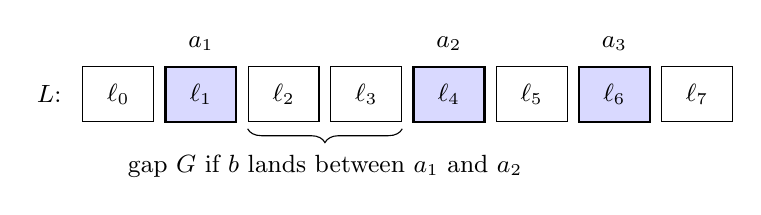
\begin{tikzpicture}[every node/.style={font=\small}, box/.style={draw, minimum width=0.9cm, minimum height=0.7cm, inner sep=1pt}, anch/.style={box, fill=blue!15, thick}]
\foreach \i/\s in {0/box,1/anch,2/box,3/box,4/anch,5/box,6/anch,7/box} {
  \node[\s] (l\i) at (\i*1.05, 0) {$\ell_\i$};
}
\node[left=4pt of l0] {$L$:};
\draw[decorate, decoration={brace, amplitude=5pt, mirror}] ($(l2.south west)+(0,-0.08)$) -- ($(l3.south east)+(0,-0.08)$) node[midway, below=6pt] {gap $G$ if $b$ lands between $a_1$ and $a_2$};
\node[above=2pt of l1] {$a_1$}; \node[above=2pt of l4] {$a_2$}; \node[above=2pt of l6] {$a_3$};
\end{tikzpicture}
\caption{Anchors (shaded) are the user's ranked Bevs most similar to the new Bev. Phase 1 binary-searches the anchors only; Phase 2 searches the gap between the two anchors the new Bev landed between.}
\end{figure}

\begin{theorem}[Properties of anchored placement]\label{thm:anchored}
Against a consistent oracle with true slot $t$ in $L$:
\begin{enumerate}[label=(\roman*)]
\item the returned index is $t$, and lies in $\{0, \dots, n\}$ for any sequence of answers;
\item every logged comparison agrees with the final index in the sense of Proposition~\ref{prop:log};
\item at most $\ceil{\log_2(k+1)} + \ceil{\log_2(g+1)}$ questions are asked, the first $\ceil{\log_2(k+1)}$ of them against Bevs of the most similar tier; if the gap is empty no cross-category question is asked at all;
\item the first question is always against a Bev of the most similar non-empty tier.
\end{enumerate}
\end{theorem}
\begin{proof}
(i) Consistency on $L$ implies consistency on the subsequence $A$ with true anchor slot $j^\ast$ such that $p_{j^\ast} < t \le p_{j^\ast+1}$ (with the conventions $p_0 = -1$, $p_{k+1} = n$), so Phase 1 returns $j^\ast$ by Theorem~\ref{thm:correctness} and $t \in [\mathrm{lo}, \mathrm{hi}]$. The gap $G$ is exactly $\ell_{\mathrm{lo}}, \dots, \ell_{\mathrm{hi}-1}$ and the oracle is consistent on it with true slot $t - \mathrm{lo}$, so Phase 2 returns $r = t - \mathrm{lo}$. For arbitrary answers, Phase 1 yields $j^\ast \in [0, k]$ hence $0 \le \mathrm{lo} \le \mathrm{hi} \le n$, and Phase 2 yields $r \in [0, g]$, so $\mathrm{lo} + r \in [0, n]$. (ii) A Phase 1 answer against $a_j$ constrains $j^\ast$ relative to $j$, hence the final index relative to $p_j$ in the same direction; a Phase 2 answer constrains $r$ relative to a position inside the gap. (iii) and (iv) follow from Theorem~\ref{thm:termination} applied to each phase and from the construction of $A$.
\end{proof}

\begin{remark}[Cost]
In the worst case ($k \approx n/2$, a wide gap) anchored placement asks about twice as many questions as plain binary search; in the typical case the gap between two adjacent anchors is short and the total is close to $\ceil{\log_2(n+1)}$. The product requirement, that the like-for-like questions come first, is met exactly. The result keeps the existing contract (\code{insertIndex}, \code{expectedBucketSize}, \code{comparisons}), so \code{submit\_ranking} is unchanged; the app needs each bucket Bev's category and brand (today \code{listBucket} returns ids only). An alternative, per-category lists with no cross-category questions at all, would give up the single comparative order behind \eqref{eq:score}; anchored placement is preferred for that reason.
\end{remark}

\subsection{Taste Profile}\label{sec:taste}

The session defined the Taste Profile as ``your average score of cafe drinks could be this number out of 10'' and ``you prefer these kinds of drinks''.

\begin{definition}[Taste Profile]
For user $u$ the profile is the table $\{(c, n_{u,c}, \mu_{u,c}, \aff_{u,c}) : n_{u,c} \ge 1\}$ ordered by $\mu_{u,c}$ descending. The display uses the raw means (what the user recognises); recommendations keep using $\aff$ (comparable across users). A preference statement ``prefers $c$ over $c'$'' is shown when $n_{u,c}, n_{u,c'} \ge 3$ and $\mu_{u,c} - \mu_{u,c'} \ge 1$.
\end{definition}

The table \code{user\_category\_stats} holds exactly this, written by \code{refresh\_user\_category\_stats} after every ranking write and nightly for everyone (A-11, 20261019000100; means and $\aff$ stored to three decimals), and read through \code{get\_taste\_profile}, which returns the rows with $n_{u,c} \ge 1$ ordered by $\mu_{u,c}$ descending, then the category's sort order, then its id. The pgTAP suite checks the stored rows against the ``five rankings'' case of \code{user-stats.vectors.json}.

\subsection{Bev of the day and Bev of the week}\label{sec:bevof}

\begin{definition}[Period winner]
Fix the zone America/New\_York (``strictly New York City''). For a period $P$ (a local calendar day, or an ISO week) let $R_P$ be the rankings created in $P$ and $B_P = \{ b : \exists\, r \in R_P \text{ with Bev } b \}$ the Bevs ranked in $P$. The winner is
\begin{equation}\label{eq:bevof}
b^\ast_P = \argmax_{b \in B_P} \bigl(\mathrm{bayes}_b,\ \abs{R_P(b)},\ n_b,\ -\mathrm{name}(b)\bigr)
\end{equation}
in lexicographic order, then the Bev's id, where $\abs{R_P(b)}$ is the number of rankings of $b$ in $P$ and $\mathrm{bayes}_b$ is the Bev's current Bayesian score \eqref{eq:bayes} with the global prior. Candidates are the active Bevs the viewer may see (the age gate applies) and there is no $\textsc{min\_raters}$ gate, so one ranking today can win. Decided 2026-10-18 (D-02): if $B_P = \emptyset$, show the winner of the most recent non-empty period with its date, flagged as not current (\code{bev\_of\_period\_at}, 20261018000100, which the pgTAP suite pins on a fixed clock).
\end{definition}

\begin{remark}
Using the current $\mathrm{bayes}_b$ rather than only the period's scores keeps the card consistent with the leaderboard the user can open, and lets a single ranking today surface a Bev while the prior still tempers it. The alternative, a period-local shrunk mean $(C m + \sum_{r \in R_P(b)} s_r)/(C + \abs{R_P(b)})$, rewards what was \emph{said} today rather than what is \emph{good}; it is one line to switch.
\end{remark}

\subsection{Likes and the Explore ranking}\label{sec:likes}

\begin{definition}[Like count and scope]
$\ell_p \in \N$ is the number of distinct users who liked post $p$. For user $u$ with follow set $F(u)$, the Explore scope is the second hop only, $E(u) = \bigl(\bigcup_{v \in F(u)} F(v)\bigr) \setminus (F(u) \cup \{u\})$: strangers whose posts the feed does not already show. Decided 2026-10-19 (D-01, D-15): while Bevi has fewer than $20$ profiles the scope widens to every user outside $F(u) \cup \{u\}$, and Explore posts are read-only (no likes, counts or comments are shown).
\end{definition}

\begin{definition}[Hotness]
For a post $p$ created at $t_p$, viewed at time $t$, with age $h = (t - t_p)$ in hours and gravity $\gamma_{\mathrm{hot}} = 1.5$,
\begin{equation}\label{eq:hot}
\hot(p, t) = \frac{\ell_p + 1}{(h + 2)^{\gamma_{\mathrm{hot}}}} .
\end{equation}
Explore lists the posts of $E(u)$ from the last $14$ days by $\hot$ descending, then post id descending, with $t$ the server's clock (never a caller parameter, so the like counts cannot be read off by moving it) and $h$ clamped at $0$ for a future-dated post (\code{explore\_hotness} and \code{get\_explore}, 20261019000400). ``Bevs getting the most likes'' over a window $W$ is $\mathrm{pop}_W(b) = \sum_{p \in W,\ \mathrm{bev}(p) = b} \hot(p, t)$; not built, since no screen asks for it yet.
\end{definition}

\begin{proposition}
$\hot$ is increasing in likes and decreasing in age; a post with $\ell$ likes outranks a post with $\ell'$ likes that is $\Delta$ hours younger iff $(\ell + 1)/(\ell' + 1) > \bigl((h+2)/(h - \Delta + 2)\bigr)^{\gamma_{\mathrm{hot}}}$. With $\gamma_{\mathrm{hot}} = 1.5$ a day-old post needs about $2.5$ times the likes (plus one) of a twelve-hour-old post to stay level.
\end{proposition}
\begin{proof}
Direct from \eqref{eq:hot}; the numeric example is $((24+2)/(12+2))^{1.5} \approx 2.53$.
\end{proof}

\subsection{Smart Recommend on the map}\label{sec:smart}

Parked by the session's guardrail (``too many features'') but specified so it can be built when wanted.

\begin{definition}[Venue score]
A venue $v$ carries a set of Bevs $M(v)$ (for chains, a shared assortment per chain plus venue-specific items). With category filter $F \subseteq C$ and untried set $\bar R(u) = B \setminus R(u)$,
\begin{equation}\label{eq:venue}
\mathrm{score}(u, v; F) = \max\bigl\{\, \shat_{u,b} : b \in M(v) \cap \bar R(u),\ \cat(b) \in F,\ \conf_{u,b} \ge 0.25 \,\bigr\},
\end{equation}
or $-\infty$ if the set is empty. Smart Recommend shows exactly the venues with $\mathrm{score}(u, v; F) \ge \theta$, with $\theta = 7$ (the \textsc{loved} threshold), and sorts them by score.
\end{definition}

The maximum (rather than a mean) answers the question the user asks on a map, ``is there something here I would love?'', and inherits the lock rule of Section~\ref{sec:predict} so low-confidence guesses never light up a venue.

\subsection{Nutrition normalisation}\label{sec:nutrition}

A vision model reads the label photo into per-serving facts $x = (x_1, \dots, x_d)$ (calories, fat, sodium, carbohydrate, sugars, protein, caffeine, \dots) together with the serving volume $V$ in millilitres.

\begin{definition}[Per 100 ml]
$x^{(100)}_i = 100\, x_i / V$. Per-container values multiply $x_i$ by the number of servings per container.
\end{definition}

\begin{definition}[Acceptance checks]
An extraction is accepted when all values are non-negative, $\text{sugars} \le \text{carbohydrate}$, $\text{added sugars} \le \text{sugars}$, $V > 0$, and the energy identity holds within tolerance:
\[
\abs{\text{calories} - (4\,\text{carbohydrate} + 4\,\text{protein} + 9\,\text{fat})} \le \max(10,\ 0.15\cdot \text{calories}).
\]
Otherwise the result is stored as \emph{needs review} and nothing is shown.
\end{definition}

Nutrition is shown on the Bev's own page to whoever opens it, never in the feed or in rankings (the session: ``just for the user themselves to see'').

\subsection{Duplicate detection and merging}\label{sec:duplicates}

\begin{definition}[Duplicate score]
For a query $q$ (name, brand, category, vessel) and an existing Bev $b$, with trigram similarity $\mathrm{tri}$ (\code{pg\_trgm}) over the normalised ``brand name'' text and its aliases,
\begin{equation}\label{eq:dup}
d(q, b) = \max\bigl(\mathrm{tri}(q, b), \max_{a \in \mathrm{aliases}(b)} \mathrm{tri}(q, a)\bigr) + 0.15\,\ind{\mathrm{brand}(q) = \mathrm{brand}(b)} + 0.10\,\ind{\cat(q) = \cat(b)},
\end{equation}
and $d(q, b) = 1$ whenever both carry the same UPC. ``Did you mean\dots'' shows the top five with $d \ge 0.3$ (the \code{pg\_trgm} default); a user-flagged duplicate with $d \ge 0.6$ is queued for merge review, below that for manual review.
\end{definition}

\begin{definition}[Merge]
Merging $b_{\mathrm{src}}$ into $b_{\mathrm{dst}}$: for each user who ranked both, keep the ranking with the better (bucket, position) and remove the other; re-point remaining rankings, aliases and Want to Try rows; recompute statistics; set $b_{\mathrm{src}}$ to status \emph{merged} with \code{merged\_into} $= b_{\mathrm{dst}}$.
\end{definition}

\begin{proposition}
A merge preserves, for every user, the relative order of all Bevs other than the merged pair, and every stored score remains inside its band.
\end{proposition}
\begin{proof}
Removal of one ranking followed by re-spacing is a monotone relabelling of positions in that bucket (Proposition~\ref{prop:score}(ii)); other buckets are untouched; band membership is Proposition~\ref{prop:score}(i).
\end{proof}

Status: the ``Did you mean\dots'' step is live as \code{find\_similar\_bevs}, which uses the trigram part of \eqref{eq:dup} (the maximum over the Bev's text and its aliases) with the category as a filter rather than a bonus; the brand and category bonuses, the duplicate report and \code{merge\_bev} are the S-13 plan.

Vessels (can, glass bottle, plastic bottle) are \emph{not} distinct Bevs and must never enter the name: the natural key is (category, brand, name, flavour). A genuinely different product (Mexican Coca-Cola, cane sugar, glass) is its own Bev with its own icon.

\subsection{One ranking per Bev per user}\label{sec:binary}

The ranking relation is a partial function $U \times B \rightharpoonup [0, 10]$: a user has or has not ranked a Bev, and if so holds exactly one score. Re-ranking \emph{updates} this value (and re-spaces the old and new buckets); it never appends. Consequently $n_b$ counts people, not drinks, and ``how many times you drank it'' is deliberately not a quantity in this system (session decision; the database enforces it with a unique constraint on (user, Bev)).

\section{Implementation notes, divergences and versioning}\label{sec:impl}

\begin{implnote}[Where the maths runs]
\code{@bevi/ranking} is pure TypeScript with no I/O or clock; Postgres holds \emph{twins} of the formulas that touch stored data (re-spacing, statistics, Bayesian score, rank points, streaks) and the two are held equal by the golden vectors in \code{shared/fixtures} (one \code{*.vectors.json} file per formula), regenerated with \code{npm run vectors} on every \code{RANKING\_VERSION} bump. Predictions and recommendations run in the client over the snapshot returned by \code{get\_prediction\_snapshot()} (decided 2026-10-12; revisit at about 200 users or a 1 MB snapshot).
\end{implnote}

\begin{implnote}[Prior mean]\label{impl:prior}
\code{bayes\_prior(p\_category\_id)} (20261019000200, \#112) is the SQL twin of \code{globalPrior} and \code{categoryPrior}: a category's own mean at $30$ rankings, else the global mean, and $5.0$ on an empty system; \code{get\_bev\_leaderboard} uses it, so a Water on the water board now shrinks toward Water's mean. Still different: \code{get\_feed} (20261014000300), \code{get\_user\_feed} (20261018000300), \code{get\_explore} (20261019000400) and \code{bev\_of\_period\_at} (20261018000100) read \code{coalesce((select mean\_score from global\_stats), 0)}, so on a system with no rankings their prior is $0$ rather than $5.0$; invisible in production, where \code{global\_stats.rating\_count > 0}. The global branch everywhere reads \code{global\_stats.mean\_score}, a \code{numeric(5,3)} refreshed every $15$ minutes, while \code{bayes\_prior}'s category branch is live and exact. \code{refresh\_global\_stats} writes \code{bev\_stats.bayes\_score} with the global prior by design (one number per Bev), but updates only rows with \code{rating\_count > 0}, so when a Bev's last ranking is removed the old figure stays in the column until the Bev is ranked again.
\end{implnote}

\begin{implnote}[Name order; resolved in 1.3.0]\label{impl:codepoints}
\code{get\_bev\_leaderboard} has ordered by \code{bayes desc, rating\_count desc, name collate "C", id} since 20261019000200, the order of Section~\ref{sec:bayes}; the earlier ``Bayesian score only'' divergence is closed, and \code{user\_category\_stats.affinity\_z} has had a writer since 20261019000100 (A-11). The last difference, on the TypeScript side, is closed in \code{RANKING\_VERSION} 1.3.0 (M-28). \code{leaderboardOrder} compared names with JavaScript \code{<}, which orders UTF-16 code units, whereas \code{collate "C"} orders code points, so the two disagreed when one name had a character outside the Basic Multilingual Plane and the other a character in U+E000--U+FFFF at the same position (an emoji against a private-use or specials character). \code{compareCodePoints} in \code{bayesian.ts} now compares a code point at a time, \code{starter.ts} reuses it for its tie-breaks, and \code{bayesian.vectors.json} gained a case with such a pair. Every catalogue name is ASCII, so no existing order changed.
\end{implnote}

\begin{implnote}[Streak history in SQL]\label{impl:streak}
\code{touch\_streak} (20261011000700) recomputes $D_u$ from \code{rankings.ranked\_at}. A re-rank deletes the row and re-inserts it with \code{ranked\_at = now()}, and a removal deletes it, so the original day leaves $D_u$ whenever it held no other ranking; \code{feed\_events} cascades on the same delete, and \code{comparisons} rows exist only when a question was asked. Section~\ref{sec:rank} counts ranking events, so after such a re-rank or removal the SQL current and longest streaks can be shorter than the specification's. Fix: an append-only ranking-event log (user, Bev, kind, timestamp) written by \code{submit\_ranking} and \code{rerank\_bev} and never deleted, which \code{touch\_streak} reads; the \code{streakFromTimestamps} cases of \code{streak.vectors.json} are its test.
\end{implnote}

\begin{implnote}[Comparison log]\label{impl:logcheck}
\code{submit\_ranking} and \code{rerank\_bev} check $\mathrm{insertIndex} \in [0, \code{expectedBucketSize}]$ and the list length, and store every comparison with its tie flag, but do not re-check Proposition~\ref{prop:log} against the submitted index. The log is a record, not yet a constraint: a client bug could store an inconsistent log without being rejected.
\end{implnote}

\begin{implnote}[Stored precision]\label{impl:precision}
Stored scores are exact (\code{numeric(4,2)} is cents$/100$). Aggregates are rounded on storage: \code{bev\_stats.avg\_score}, \code{score\_stddev} and \code{bayes\_score} to two decimals; \code{user\_stats}, \code{user\_category\_stats} and \code{global\_stats.mean\_score} to three. \code{bayes\_score} is computed from the exact \code{sum\_score}, not from the rounded mean. The live leaderboard, feed and Explore figures are unrounded \code{numeric}; \code{bev\_of\_period\_at} returns two decimals. The prediction snapshot computes user statistics live, so the client's z-scores are exact. The golden vectors are compared unrounded at $10^{-6}$ in TypeScript and at column scale in pgTAP.
\end{implnote}

\begin{implnote}[What pgTAP checks against the vectors]\label{impl:vectors}
\code{08\_taste\_profile} pins one case of \code{user-stats.vectors.json}; \code{09\_leaderboard\_parity} pins \code{bayes\_prior} and the full leaderboard order on its own fixture, including the \code{collate "C"} tail; \code{07\_bev\_of\_period} pins Section~\ref{sec:bevof} on a fixed clock; \code{10\_explore} pins one value of \eqref{eq:hot}. No SQL test runs \code{score-from-position.vectors.json} against \code{ranking\_score}, \code{bev-stats.vectors.json} against \code{stddev\_pop}, the \code{bayesianAverage} cases against \code{bayes\_score}, \code{streak.vectors.json} against \code{touch\_streak} (the timezone cases are where the engines could differ) or \code{rank-points.vectors.json} against \code{user\_rank\_points}. Those are the gaps to close in A-14's follow-up.
\end{implnote}

\begin{implnote}[Exploration slots]
The development document lists the three slots for a 20-item list as 4, 9, 15; the implemented even-spacing rule \eqref{eq:slots} gives 4, 9, 14. The code is the specification here.
\end{implnote}

\begin{center}
\begin{tabular}{@{}llp{9.5cm}@{}}
\toprule
Version & Date & Change \\
\midrule
1.0.0 & 2026-10-09 & First vectors: bands 7/4, placement, exact cents, statistics, Bayesian average, rank points, streaks \\
1.1.0 & 2026-10-11 & Prediction snapshot, Layers 1--2, blend, exploration, starter set \\
1.2.0 & 2026-10-14 & Bev-graph edge weights: tree \eqref{eq:wp}, profile \eqref{eq:prof} and embedding similarity, $w$ \eqref{eq:w}, top-$K_E$ selection, as \code{edges.vectors.json} (M-24); earlier vectors unchanged apart from the header \\
1.3.0 & 2026-10-24 & Taste formulas of Section~\ref{sec:tastegraph} (M-28): Pearson over the common subset \eqref{eq:pearson}, taste vectors \eqref{eq:taste}, attribute similarity, the blend \eqref{eq:blendsim}, neighbour selection and reliability, as \code{graph.vectors.json}. Layer~2 gains \code{userSimilarity: 'pearson'}, default \code{'cosine'}, so live predictions are unchanged; $w$ is unchanged. Fix: leaderboard and starter-set names now compare by Unicode code point as Section~\ref{sec:bayes} specifies, which resolves Implementation note~\ref{impl:codepoints} (they compared UTF-16 code units, which put astral characters before U+E000--U+FFFF), with one new \code{leaderboardOrder} vector; ASCII names, hence every catalogue name, order as before. Earlier vectors unchanged apart from the header; current \\
(next) & --- & Anchored placement (Section~\ref{sec:anchored}) when adopted; requires a bump and new vectors \\
\bottomrule
\end{tabular}
\end{center}

\appendix

\section{Constants}\label{app:constants}

All values from \code{packages/ranking/src/constants.ts}, \code{RANKING\_VERSION} 1.3.0.

\begin{center}
\small
\begin{tabular}{@{}p{5.1cm}p{2.7cm}p{6.6cm}@{}}
\toprule
Constant & Value & Role \\
\midrule
\code{BANDS} & $[0,4]$, $[4,7]$, $[7,10]$ & Score bands for \textsc{disliked}, \textsc{fine}, \textsc{loved}; the first two exclude their top edge \\
\code{SIGMA\_FLOOR} & 1.0 & Floor on any standard deviation used for z-scores \\
\code{MIN\_N\_USER} & 3 & Below this a user's z-scores use global statistics; predictions withheld \\
\code{MIN\_N\_CAT} & 3 & Below this \code{effectiveCategoryStats} falls back to the user's overall statistics; exported and in the vectors, but the product shows raw category means (Section~\ref{sec:taste}) \\
\code{GLOBAL\_FALLBACK} & $(5.0, 2.5)$ & Only when the system has no rankings \\
\code{K\_AFF} & 2 & Shrinkage of category affinity \\
\code{K\_G} & 3 & Shrinkage of a Bev's normalised global score \\
\code{BAYES\_C} & 3 & Prior weight of the Bayesian average (raise to 5 when median $n_b > 10$) \\
\code{BAYES\_CATEGORY\_PRIOR\_MIN} & 30 & Rankings a category needs before its own mean is the prior \\
\code{MIN\_RATERS} & 2 & Leaderboard eligibility \\
\code{SIM\_WEIGHTS} & 0.40 / 0.30 / 0.20 / 0.10 & Category, brand, flavour tokens, price tier \\
\code{SIM\_MIN} & 0.1 & Pairs below this are dropped \\
\code{PRICE\_TIER\_SPAN} & 3 & Largest $\abs{\mathrm{tier} - \mathrm{tier}'}$ (tiers 1--4) \\
\code{LAYER1\_WEIGHTS} & 0.40 / 0.40 / 0.20 & Affinity, content, global \\
\code{CONF1\_USER\_N},\newline \code{CONF1\_MASS} & 10, 4 & Layer 1 confidence saturation \\
\code{CF\_K} & 10 & Neighbours per prediction \\
\code{CF\_MIN\_COMMON} & 2 & Minimum common items for a non-zero user similarity \\
\code{CF\_SIGNIFICANCE} & 5 & Significance weighting of user similarity \\
\code{LAMBDA\_MAX},\newline \code{LAMBDA\_USER\_N} & 0.7, 15 & Blend weight ceiling and user-history saturation \\
\code{CONFIDENCE\_LOCK} & 0.25 & Below this the UI shows a lock \\
\code{EPSILON} & 0.15 & Share of the list given to exploration \\
\code{JITTER\_SD} & 0.15 & Ordering-only jitter (z-units) \\
\code{RECOMMEND\_N} & 20 & Default list length (API caps at 50) \\
\code{STARTER\_K},\newline \code{STARTER\_CORE} & 10, 6 & Onboarding set size and shared core \\
\code{STARTER\_MAX\_PER\_CATEGORY},\newline \code{STARTER\_MIN\_CATEGORIES} & 2, 5 & Spread of the onboarding set \\
\code{RANK\_POINTS\_WEIGHTS} & 1 / 3 / 2 & Bevs ranked, current streak, adopted Bevs created \\
\code{STREAK\_PERIOD} & day & Daily streak (weekly is a constant change) \\
\bottomrule
\end{tabular}
\end{center}

\begin{center}
\small
\begin{tabular}{@{}p{5.1cm}p{2.7cm}p{6.6cm}@{}}
\toprule
Constant & Value & Role \\
\midrule
\code{EDGE\_WEIGHTS} & 0.25 / 0.15 / 0.30 / 0.30 / 0 & Tree, content, embedding, profile, co-preference \eqref{eq:w} \\
\code{EDGE\_TOP\_K},\newline \code{EDGE\_MIN\_WEIGHT} & 20, 0.3 & Edges kept per Bev ($K_E$) and their minimum weight \\
\code{PROFILE\_WEIGHTS} & 0.40 / 0.15 / 0.10 / 0.05 / 0.15 / 0.15 & Base, carbonation, dairy, alcohol, caffeine, sweetness \eqref{eq:prof} \\
\code{PROFILE\_LEVEL\_SPAN} & 3 & Largest caffeine or sweetness difference \\
\code{TASTE\_K} & 2 & Shrinkage $K_T$ of a taste-vector entry \eqref{eq:taste} \\
\code{TASTE\_MIN\_ATTR\_BEVS} & 2 & Catalogue Bevs an attribute needs to be kept \\
\code{TASTE\_ALPHA} & 0.5 & Pearson weight $\alpha$ of the blend \eqref{eq:blendsim} when $m \ge 2$ \\
\code{TASTE\_SHARED\_MIN},\newline \code{TASTE\_MIN\_SHARED\_ATTRS} & 0.2, 2 & $\abs{t}$ for a shared attribute; bridging attributes an attribute-only pair needs \\
\code{TASTE\_BRIDGE\_KINDS} & brand, flavour & Attribute kinds that bridge (categories do not) \\
\code{TASTE\_SIM\_FLOOR},\newline \code{TASTE\_NEIGHBOUR\_K} & 0.1, 25 & Least similarity kept and neighbours kept per user in \code{user\_neighbors} \\
\code{NEIGHBOUR\_RELIABILITY\_N} & 15 & $N_0$ of the reliability weight $\min(1, n_v/N_0)$ (chosen; the doc leaves it open) \\
\bottomrule
\end{tabular}
\end{center}

\section{Symbols}

\begin{center}
\small
\begin{tabular}{@{}lp{10cm}@{}}
\toprule
Symbol & Meaning \\
\midrule
$U, B, C$ & Users, Bevs, categories; $\cat(b)$ the category of $b$ \\
$R(u), R^{-1}(b)$ & Bevs ranked by $u$; users who ranked $b$ \\
$n_u, n_b, n_{u,c}$ & Counts of rankings by user, of a Bev, by user within a category \\
$s_{u,b}$ & Stored score of $u$ for $b$ (two decimals) \\
$\sigma(i, n)$ & Score of position $i$ in a bucket of $n$ (eq.~\ref{eq:score}) \\
$\mu^\ast_u, \sigma^\ast_u$ & Effective mean and (floored) standard deviation of $u$ \\
$z_{u,b}$ & Normalised score of $u$ for $b$ \\
$\aff_{u,c}$ & Category affinity (eq.~\ref{eq:aff}); $g_b$ normalised global score (eq.~\ref{eq:g}) \\
$\mathrm{bayes}_b$ & Bayesian leaderboard score (eq.~\ref{eq:bayes}); $m$ its prior mean, $C$ its weight \\
$\simi(b, b')$ & Content similarity; $\simi'(u, v)$ significance-weighted user similarity \\
$\rho, \rho', t_u, \simi_A, \simi_B$ & Pearson and shrunk Pearson user similarity, taste vector, attribute and blended user similarity (Section~\ref{sec:tastegraph}) \\
$\zhat^{(1)}, \zhat^{(2)}, \zhat$ & Layer 1, Layer 2 and blended predictions in z-units; $\shat$ in score units \\
$\lambda, \supp, \conf$ & Blend weight, neighbour support, confidence \\
$\simi_T, w$ & Tree similarity and Bev-graph edge weight (Section~\ref{sec:anchored}) \\
$A, G, k, g$ & Anchors, gap, and their sizes in anchored placement \\
$\hot(p, t)$ & Time-decayed popularity of a post (eq.~\ref{eq:hot}) \\
\bottomrule
\end{tabular}
\end{center}

\end{document}
